\chapter{Blind GNSS Search of Extraterrestrial EUV Sources}

In the previous chapter we saw that an algorithm for detecting the location of an EUV source (in this case, the Sun) is possible with a first, brute force approach. Here, the algorithm is studied in more detail considering different possible methods to increase its precision and several optimizations are presented aiming to reduce its computational complexity.

\section{Mean VTEC as a reliable indicator of the moment of the flare}

In the previous chapter, before doing any computations regarding the correlation between the VTEC and solar-zenith angle we had to find the moment of the flare we wanted to study. This was done using a simple approach: computing the mean VTEC value for each epoch and assuming the one with the highest mean was the moment of the flare.

To see if the mean VTEC could be used as a reliable indicator, the algorithm was tested with all available epochs of the data set, in order to study the effect of this indicator in the resulting estimation of the source's location.

To do this we ordered the different epochs available in our data set by their mean VTEC, inserting them into a priority queue. \\

Figure \ref{fig:differentEpochs} shows the evolution of the correlation coefficient of the best estimated location (a) and its total error (right ascension error + declination error) (b) as the mean VTEC of the epoch decreases.

\clearpage

\begin{figure}[!htb]
	\begin{subfigure}[b]{0.5\textwidth}
		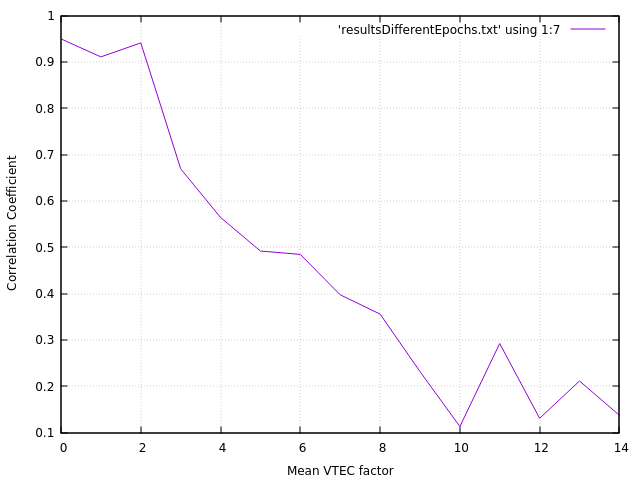
\includegraphics[width=\linewidth]{images/ch6/spikes/correlationDecrease.png}
		\caption{Correlation coefficient}
	\end{subfigure}
	\hfill
	\begin{subfigure}[b]{0.5\textwidth}
		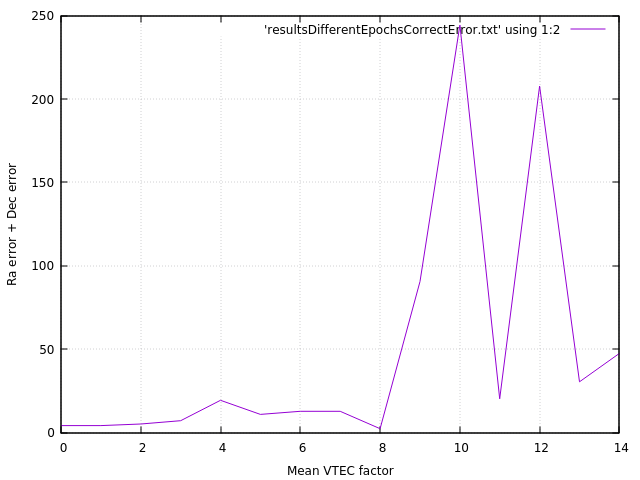
\includegraphics[width=\linewidth]{images/ch6/spikes/decreaseRangeError.png}
		\caption{Error of the estimated source}
	\end{subfigure}
	\caption{Correlation and error of the solution as the mean VTEC decreases}
	\label{fig:differentEpochs}
\end{figure}

As we can see, the correlation rapidly decreases from 1 (almost linear) to a negative coefficient. The error, on the other hand, doesn't experience much change for the first epochs but finally increases considerably. 

The fact that the error remains near 0 as the correlation rapidly decreases for the first epochs can be due to the fact that different location of the source reduces its effect on the  the estimated location with the highest correlation coefficient is still similar to that of the source. As the position of the source changes (the Sun in this case)  TODO: este parrafo

\section{Linear fitting: discarding outliers}

Explicar q los ultimos al cortar el vtec no iba bien, el problema? antes 1 sola pasada por los valores, ahora, 1 para calcular cos, otras por iteraciones y una iltima para la correlacion

poner ejemplo decrease range, 1 caso, mismos params -> diff tiempo

\section{Decreasing the range of the search}

As we saw in the previous chapter, to increase the precision of the algorithm, the \textit{step} with which we iterate over the possible angles (right ascension and declination) is reduced. This causes more possible Suns to be considered. For example, with a step of one degree, we consider all possible right ascensions [0,360] and declinations [-90,90] which is  $360*180 = 64800$ Suns, minus the $2*360 - 2 = 718$ right ascensions we don't consider because as we have seen right ascensions for declinations of -90 and 90 are the same location.

We want to have the highest precision possible without having to consider all $64800 - 718 = 64082$ possibilities by progressively reducing the search range. 

\subsection{Pseudocode}

This first optimization works as follows: the entire possible range is considered with a large starting step (e.g 60). Once the best Sun is found within this range, the precision is increased (the step is decreased) and the search range is reduced. This way the precision is increased but the number of considered possibilities remains similar each iteration of the algorithm. The following is the pseudocode\footnote{The code for the special cases of -90 and 90 degree declinations is not included for more readability. It is included in the implantation, in the following section.} for the algorithm using this optimization:

\begin{algorithm}
	\caption{Search range decrease}\label{searchRangeDecrease}
	\begin{algorithmic}[1]
		\Procedure{main}{}
		\State $\textit{epoch} \gets \text{findSpikeInData()}$ 
		\State $\text{filterDataByEpoch(\textit{epoch})}$
		\State $bestSun \gets nil$
		\State $r \gets \text{defaultRange()}$ 
		\For {$step = initStep; step >= min; step\ /= 2$}
		\For {$ra = r.lowerRa;\ ra <= r.upperRa;\ ra += step$}
		\For {$dec = r.lowerDec;\ dec <= r.upperDec;\ dec += step$}
		\State $currentSun \gets computeCorrelationPossibleSun(ra, dec)$
		\If {$currentSun.correlation > bestSun.correlation$} 
		\State $bestSun \gets currentSun$
		\State $r \gets \text{newRange(\textit{bestSun, step})}$ 
		\EndIf
		\EndFor
		\EndFor
		\EndFor
		\\
		\Return $bestSun$
		\EndProcedure
	\end{algorithmic}
\end{algorithm}

A very important part of the algorithm is computing the correlation. In the previous chapter we didn't consider discarding outliers from our data set because it appeared that considering all samples yielded good results, but testing with a different flare resulted in problems because of that. That is why in the previous section a method for discarding outliers was introduced. \\

The main problem of discarding outliers is that while before we the correlation could be computed with a single pass, multiple are needed to be able to discard outliers.
This is explained in more detail in the next chapter, along with the time comparison and error of both possibilities (discarding outliers or not).

\subsection{Implementation}

This first piece of code is the main loop of the method, which starts with a default range of ra=[0, 360], dec=[-90, 90] and reduces it every iteration based on the current best Sun's estimated location. 

Furthermore, because an increase in the precision of the tested location doesn't necessarily imply an improvement in the solution, the new candidate is inserted into a \textit{priorityQueue} ordered by the coefficient to assure that the method returns the best one found throughout the entire loop. 

\begin{minipage}{\linewidth}
	\begin{lstlisting}[language=c, caption=Decreasing the range and increasing the precision]
void TraverseGlobe::decreasingSTEP() {
	int rangeSize = 3;
	int initStep = 60;
	possibleSunInfo currentSun;
	searchRange range = setRange(currentSun, true, initStep, rangeSize);
	for (double step = initialStep; step >= 0.5; step /= 2) {
		currentSun = considerPossibleSuns(step, range, plotData);
		bestSuns.push(currentSun);
		range = setRange(currentSun, false, step, rangeSize);
	}
}\end{lstlisting}
\end{minipage}

The \textit{setRange} function sets a new range based on the estimated location that depends on the precision used for the values and assure that valid value is returned.

\begin{minipage}{\linewidth}
	\begin{lstlisting}[language=c, caption=Setting the new range based on the estimated source location]
searchRange setRange(possibleSunInfo sun, bool defaultR, double step, int rangeSize) {
	searchRange range;
	if (defaultR) {
		range.lowerRa = 0;
		range.upperRa = 360;
		range.lowerDec = -90;
		range.upperDec = 90;
	}
	else {
		double raRange = step*rangeSize;
		double decRange = step*rangeSize;
		range.lowerRa = sun.ra - raRange >= 0 ? sun.ra - raRange : 0;
		range.upperRa = sun.ra + raRange <= 360 ? sun.ra + raRange : 360;
		range.lowerDec = sun.dec - decRange >= -90 ? sun.dec - decRange : -90;
		range.upperDec = sun.dec + decRange <= 90 ? sun.dec + decRange : 90;
	}
	return range;
}\end{lstlisting}
\end{minipage}

Finally, the \textit{considerPossibleSuns} function has the same functionality than the one from the previous chapter, it iterates over the possible locations, this time, however, it does so over the given range, rather than just the default one. 

The names of the lower and upper bound variables have been changed (\textit{uRa} instead of \textit{upperRa}, for example) for readability.

\begin{minipage}{\linewidth}
	\begin{lstlisting}[style=myCStyle, caption=Iterating over possible locations within the given range]
possibleSunInfo considerPossibleSuns(double step, searchRange range) {
	FortranController fc;
	double pearsonCoefficient;
	int i = 0;
	possibleSunInfo bestSun;
	bestSun.coefficient = -23;
	bestSun.location = "salu2";
	
	for (double dec = range.lDec; dec <= range.uDec; dec += step) {
		if (dec != -90 and dec != 90) {
			for (double ra = range.lRa; ra <= range.uRa; ra += step) {
				pearsonCoefficient = fc.computeCorrelation(&ra, &dec);
				if (pearsonCoefficient > bestSun.coefficient) {
					bestSun.coefficient = pearsonCoefficient;
					bestSun.ra = ra;
					bestSun.dec = dec;
				}
			}
		}
		else {
			//Do only once
			double ra = 0;
			pearsonCoefficient = fc.computeCorrelation(&ra, &dec);
			if (pearsonCoefficient > bestSun.coefficient) {
				bestSun.coefficient = pearsonCoefficient;
				bestSun.ra = ra;
				bestSun.dec = dec;
			}
		}
	}
	return bestSun;
}\end{lstlisting}
\end{minipage}

Finally, the \textit{computeCorrelation} calls the Fortran code (the same used in the Brute Force chapter) to compute the correlation, but as mentioned before, in order to discard outliers it does so with multiple iterations over the data: first it calculates the solar-zenith angle cosine for each IPP, then it discards the outliers and finally traverses the filtered data one last time to compute the correlation:

\begin{minipage}{\linewidth}
\begin{lstlisting}[style=myCStyle, caption=Discarding outliers and computing the correlation]
double computeCorrelation(double* ra, double* dec) {
	FileManager fileManager;
	int sigma = 1;
	int iterations = 6;
	computecosinesofcurrentsourcefortran_(ra, dec);
	fileManager.discardOutliersLinearFitFortran(sigma, iterations);	
	return computecorrelationfortran_(ra, dec);
}\end{lstlisting}
\end{minipage}

Another change that could be done to improve this method's performance would be to adopt a sort of \textit{"Dynamic Programming"} strategy in order to avoid repeated calculations (the new range will always be inside the previous range). However, the problem is that because we are dealing with a different precision for the right ascension and declination values every loop, the same values are never used. TODO: justificar mejor esto? \\

Seeing the computational complexity of this method because of the fact that outliers have to be discarded, we decided to instead focus on a different method that would rely only on the data itself, instead of considering the many possible locations of the source.

\clearpage
\section{Least Squares method}

As we have seen in previous chapters the overall process to determine the location of the source is studying the correlation between the VTEC value and the solar-zenith angle (or source-zenith angle, speaking in general terms).

For this, we only had data for the VTEC and the location of the IPP. Then, given a possible source location we computed the angle between the IPP and the source, using the following equations:

\begin{equation} \label{eq:61}
unitVectorIPP =	
\begin{bmatrix}
\cos\delta_{g} * \cos\alpha_{g} \\ 
\cos\delta_{g} * \sin\alpha_{g} \\
\sin\delta_{g}
\end{bmatrix}
\end{equation}

\begin{equation} \label{eq:62}
unitVectorSource =	
\begin{bmatrix}
\cos\delta_{s} * \cos\alpha_{s} \\ 
\cos\delta_{s} * \sin\alpha_{s} \\
\sin\delta_{s}
\end{bmatrix}
\end{equation}

\begin{equation} \label{eq:63}
\cos \chi = unitVectorIPP \cdot unitVectorSource
\end{equation}\\

And then, having the VTEC and source-zenith cosine, we found the correlation of the two variables, expecting that the real source would yield a near-linear correlation.

The aim of this section's method was to do the inverse, that is, having the VTEC, location of the IPP and correlation (1, assuming a near-linear correlation), compute the location of the source.

Visually, we can see the relation between VTEC and the computed cosine in figure \ref{fig:solar-zenith-angle}, obtained in chapter 3 when studying the a specific case for the Sun.

\begin{figure}[!htb]
	\begin{centering}
		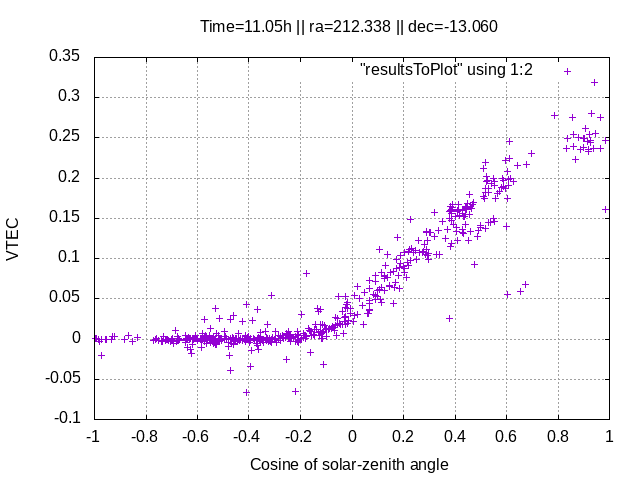
\includegraphics[width=0.5\linewidth]{images/ch4/resultSunTest.png}
		\caption{Visual representation of the solar-zenith angle}
		\label{fig:solar-zenith-angle}
	\end{centering}
\end{figure}

As we have previously seen for this case, there appears to be a linear relation starting around $\cos \chi = -0.1$ between the two studied parameters. Therefore, we could define this linear relation as follows: $\Delta V$ as a function of the cosine (\ref{eq:linearRelation}).

\begin{equation} \label{eq:linearRelation}
\Delta V = a\cos \chi + b
\end{equation}

Because the cosine is computed using the previous equations (\ref{eq:61}, \ref{eq:62}, \ref{eq:63}). The cosine can be expressed as follows:

\begin{equation} \label{eq:cosine}
\cos \chi = XX' + YY' + ZZ'
\end{equation}

Where $X'$, $Y'$, $Z'$ are the components of the IPP's unit vector obtained from equation \ref{eq:61}, and $X$, $Y$, $Z$ are the unknowns of our equation: the components of the source's unit vector, which could be used to easily find the right ascension and declination of the source by using trigonometric operations.

However, finding the value of this unknowns is the difficult part of this method. Taking the cosine as \ref{eq:cosine} we can express the linear function as:

\begin{equation} \label{eq:substitute}
\Delta V = aXX' + aYY' + aZZ' + b
\end{equation}

Because $a$ and $b$ are unknowns as well as $X$, $Y$ and $Z$, we can group them as follows:

\begin{equation} \label{eq:newNames}
\Delta V = \alpha X' +  \beta Y' +  \gamma Z' + b
\end{equation}

Our aim now would be to solve the previous equation, but then we would need to obtain only the values of $X$, $Y$ and $Z$. We can see that:

\begin{equation} \label{eq:elTrucoDelAlmendruco}
\sqrt{\alpha^{2}+\beta^{2}+\gamma^{2}} = \sqrt{a^{2}(X^{2}+Y^{2}+Z^{2})} = \sqrt{a^{2}} = a
\end{equation}

Because $X$, $Y$ and $Z$ are the components of a unit vector\footnote{$\sqrt{(X^{2}+Y^{2}+Z^{2})} = 1$}. The previous allows us to, once we know the values of $\alpha$, $\beta$ and $\gamma$, obtain $X$, $Y$ and $Z$ by doing:

\begin{equation} \label{eq:iso}
\frac{\alpha}{\sqrt{\alpha^{2}+\beta^{2}+\gamma^{2}}} = \frac{\alpha}{a} = \frac{aX}{a} = X
\end{equation} \\

In our data we can find, for each IPP: $\Delta V$, $X'$, $Y'$, $Z'$ (because we have the right ascension and declination of the point).

For each of these IPPs, we have an equation of the form $\Delta V = \alpha X' +  \beta Y' +  \gamma Z' + b$ and, therefore, we have an overdetermined system of equations, with more equations (unknown, depends on the input data) than variables (four: $\alpha$, $\beta$, $\gamma$ and $b$)

Knowing how to obtain $X$, $Y$ and $Z$ from $\alpha$, $\beta$ and $\gamma$, we can now focus on solving the system of equations to obtain the latter unknowns .

Because we have an overdetermined system of equations, the solution can be approximated using the Least Squares approach. The system can be represented in matrix form $y = AX$ as follows:

\begin{equation} \label{eq:matrixSystem}
\begin{bmatrix}
\Delta V_{0} \\ 
\Delta V_{1} \\
. \\
. \\
. \\
\Delta V_{n}
\end{bmatrix}
=
\begin{bmatrix}
X'_{0} & Y'_{0} & Z'_{0} & 1 \\ 
X'_{1} & Y'_{1} & Z'_{1} & 1 \\
. & . & . & .\\
. & . & . & .\\
. & . & . & .\\
X'_{n} & Y'_{n} & Z'_{n} & 1 \\
\end{bmatrix}
\begin{bmatrix}
\alpha \\ 
\beta \\
\gamma \\
b \\
\end{bmatrix}
\end{equation}

This way, X, the least square estimate, can be computed by:

\begin{equation}
	X = (A^{T}A)^{-1}A^{T}y
\end{equation}

\subsection{Pseudocode}

\subsection{Implementation}

When 

One of the main advantages of this method over the others is that we don't need to compute the correlation, that it is, discard outliers. (o si????)

\clearpage

\section{Other possibilities}

Here other possible optimizations are considered that could be used to, in the future, extend the algorithm and perhaps improve its performance and accuracy.

\subsection{Hill Climbing}

explicar que no es hill climbing exactamente, algo mas simple rollo greedy 
Using the previous optimization we can see a plot of all the possibilities the algorithm considers:

\begin{figure}[!htb]
	\begin{centering}
		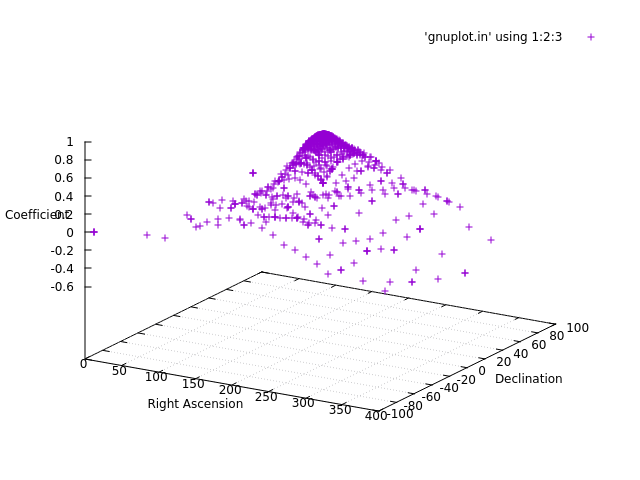
\includegraphics[width=0.5\linewidth]{images/ch6/hillClimbing/resultsAll.png}
		\caption{All visited candidates of the solution space}
		\label{fig:solutionSpace}
	\end{centering}
\end{figure}

As we can see in the previous figure, there appears to be a "hill" (our solution) so an attempt to solve the problem using a \textit{Hill Climbing} approach was also considered.

While not exactly Hill Climbing, a simple greedy algorithm was implemented as a first attempt to test if this method could yield good results:

\begin{minipage}{\linewidth}
	\begin{lstlisting}[language=c, caption=Hill Climbing]
	// Starting position
	sourceInfo current;
	current.ra = 160;
	current.dec = -20;
	int i = 0;
	// Loop with limit or until no progress can't be made
	while (++i < 100) {
	vector<sourceInfo> candidates = getNeighbourList(current);
	sourceInfo newCandidate = getBestCandidate(candidates);
	if (newCandidate < current) {
	break;
	}
	current = newCandidate;
	}
	\end{lstlisting}
\end{minipage}

The following figure shows the results of the execution for two different starting states. For both of them, the algorithm ran until it couldn't progress any further (wasn't interrupted by the iteration limit). The plots contain both the possibilities considered by the decrease range method (in purple, the same plot as \ref{fig:solutionSpace}) and the path taken by the Hill Climbing method (in green).

\begin{figure}[!htb]
	\begin{subfigure}[b]{0.5\textwidth}
		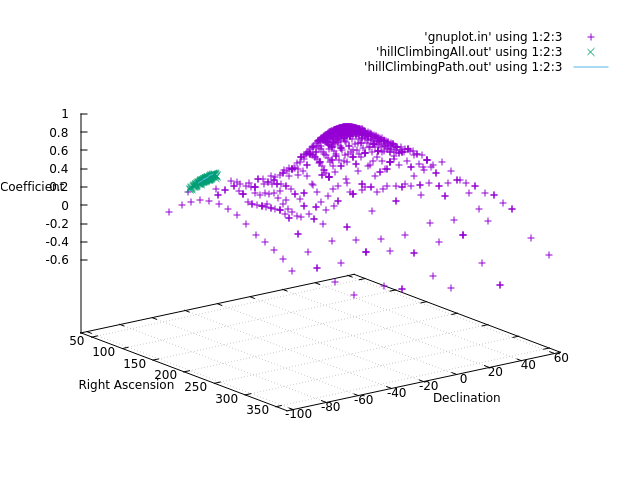
\includegraphics[width=\linewidth]{images/ch6/hillClimbing/resultsPathBad.png}
		\caption{Start: ra=100º, dec=-60º}
	\end{subfigure}
	\hfill
	\begin{subfigure}[b]{0.5\textwidth}
		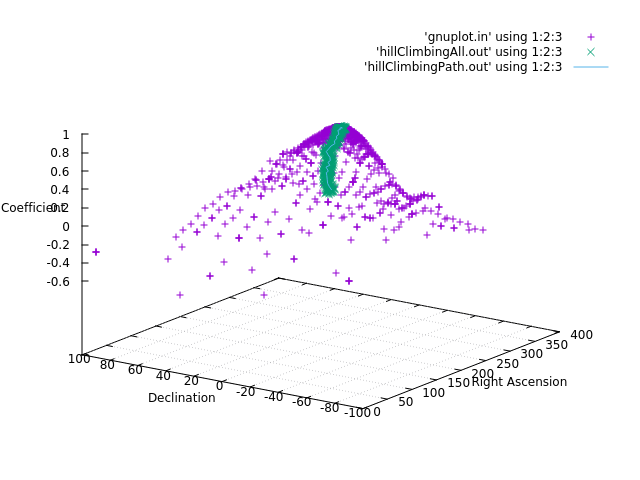
\includegraphics[width=\linewidth]{images/ch6/hillClimbing/resultsPathGood.png}
		\caption{Start: ra=160º, dec=-20º}
	\end{subfigure}
	\caption{Paths taken by the Hill Climbing algorithm}
	\label{fig:hillClimbingPaths}
\end{figure}

Visually, we can see that the number of considered possibilities is inferior and the top is reached for case (b), but a problem appears: \textbf{a local maxima}.

If we take a starting right ascension of 160º and a declination of -20º, the algorithm takes a path that gets to the top of our solution, yielding similar results to the previous, decrease range method.

However, with a starting right ascension of 100º and a declination of -60º, the algorithm finds a local maxima on its way and can't progress to the real best solution.

As a result, we can't rely on the Hill Climbing approach for all cases, considering that local maxima may exist for our type of problem. Because of this, another possibility would be to use the Simulated Annealing algorithm so that we can explore other parts of the solution space and find other paths that might lead to our desired solution, instead of only.

\subsection{Simulated Annealing}

\subsection{OpenMP}

Explicar OpenMP

\section{Discarding the Sun hemisphere}

So far the algorithm has been studied for the case of the Sun, as it is a source that should be detected more easily than far-away stars. 

The main idea is that the algorithm should detect extraterrestrial EUV sources (if possible) other than the Sun. it follows that it should, before any other computations, discard the Sun hemisphere based on the current Sun location. The greater impact of the Sun's radiation due to its proximity would blind the algorithm from detecting sources that may be having an effect on that hemisphere because of the noise.


bla bla bla

This will be used in the next chapter, in which the presented methods will tested with flares from the Sun and far-away stars.